\documentclass{article}
\usepackage[utf8]{inputenc}
\usepackage{graphicx}
\usepackage[%  
    colorlinks=true,
    pdfborder={0 0 0},
    linkcolor=black
]{hyperref}
\graphicspath{ {./images/} }
\setlength{\parindent}{0em}

\title{Relazione Progetto Sviluppo Applicazioni Mobili}
\date{Luglio 2022}
\author{Samuele Calugi\\ Corso A \\ 579086}
\begin{document}
\maketitle
\tableofcontents

\section{Introduzione}
Il progetto VoxelGO consiste nello sviluppo di un'applicazione simile a Pokémon GO: l'utente ha la possibilità di muoversi all'interno del mondo reale visualizzando 
una mappa all'interno dell'applicazione. Vengono generati casualmente dei Marker sulla mappa che segnalano la posizione di un collezionabile, ovvero di un modello
3D. 

L'utente ha quindi la possibilità di cliccare sul Marker, dopo che ha raggiunto una certa distanza dall'obiettivo e ottenere quindi il suo collezionabile. 
Quest'ul-timo viene conservato all'interno di un database dentro l'applicazione. 

Per poter mostrare i collezionabili, è stata implementata una WebView che renderizza una pagina web contentente al suo interno il modello 3D del collezionabile.
Il collezionabile può essere visualizzato soltanto dopo che l'utente è riuscito a catturarlo.

\medskip

Per riassumere, il progetto VoxelGO contiene:
\begin{itemize}
    \itemsep 0em 
    \item integrazione dei servizi di Google con le api di GoogleMaps.
    \item database interno all'applicazione per memorizzare i collezionabili e le loro catture.
    \item integrazione delle WebView con una RestAPI.
\end{itemize}

\subsection{Linguaggio di programmazione e librerie utilizzate}

L'applicazione è stata sviluppata in Java e resa disponibile su \href{https://github.com/Walrus98/voxelgo-android}{github}. Le librerie sono state implementate nel progetto con Gradle e sono facilmente visibili all'interno del
file \textbf{build.gradle}. Le librerie utilizzate sono le seguenti:
\begin{itemize}
    \itemsep 0em 
    \item \textbf{room}, utilizzata per la gestione del database all'interno dell'applicazione.
    \item \textbf{play-services-maps}, utilizzata per implementare la mappa di Google.
    \item \textbf{play-services-location}, utilizzata per acquisire la posizione dell'utente tramite i servizi di Google.
    \item \textbf{viewmodel}, utilizzata per tenere alcuni dati in memoria anche dopo la distruzione e la ricreazione di una view.
    \item \textbf{livedata}, utilizzata per osservare il cambiamento di strutture dati mutabili all'interno dell'applicazione.
    \item \textbf{lottie}, utilizzata per inserire delle view animate.
    \item \textbf{glide}, utilizzata per scaricare immagini dalla rete e per cacharle all'interno dell'applicazione.
    \item \textbf{commons-io}, utilizzata come meccanismo di IO nell'applicazione.
    \item \textbf{gson}, utilizzata per deserializzare il file JSON inviato dalla Rest.
\end{itemize}

\section{Struttura dell'applicazione}

\subsection{Activity e Fragment}

L'applicazione è stata sviluppata creando un'unica Activity. Le schermate dell'applicazione sono rappresentate dai dei Fragment. La classe
MainActivity contiene al suo interno un FrameLayout vuoto, chiamato \textbf{fragment\texttt{\_}container}. Grazie all'utilizzo del FragmentManager, 
quest'ultimo viene continuamente sostituito con uno dei Fragment dell'applicazione, in base alla schermata che si vuole mostrare sul telefono.
I Fragment presenti all'interno dell'applicazione sono:
\begin{itemize}
    \itemsep 0em 
    \item \textbf{FragmentHome}, mostra l'insieme di tutti i collezionabili che l'utente può catturare.
    \item \textbf{FragmentMap}, mostra la mappa implementata con le librerie di Google in cui l'utente può catturare i collezionabili.
    \item \textbf{FragmentProfile}, mostra i collezionabili catturati.
    \item \textbf{FragmentCollectible}, mostra il modello 3D del collezionabile catturato tramite WebView.
\end{itemize}

\subsection{Database dell'applicazione}

Il database è composto da due tabelle: 
\begin{itemize}
    \itemsep 0em 
    \item \textbf{collectibles}, contiene l'insieme di tutti i collezionabili che l'utente può catturare. 
    \item \textbf{captures}, contiene tutte le catture effettuate dall'utente
\end{itemize}

Come è possibile vedere dal codice, la struttura del database è stata implementata utilizzando la libreria room fornita da Google.
Quest'ultima prevede:
\begin{itemize}
    \itemsep 0em 
    \item la realizzazione di una classe Database, chiamata in questo caso \textbf{VoxelRoomDatabase}, che si occupa in maniera autonoma di creare
    il file \textbf{.db} e salvarlo nella memoria interna del telefono. Il file \textbf{.db} viene poi utilizzato e interpretato da SQLite. Per poter
    eseguire operazioni sul database da parti distinte dell'applicazione, è stato necessario implementare la classe \textbf{VoxelRoomDatabase} come
    Singleton. In questo modo, tale classe viene istanziata in memoria un'unica volta e viene eliminata dal GarbageCollector al momento della terminazione
    dell'applicazione. Quando è necessario interagire con il database, quindi, è sufficiente prendere il suo riferimento in memoria con il metodo \textbf{getInstance()}. 
    \item la realizzazione di una classe DAO (Data Access Object), generalmente almeno una per tabella, che contiene le query che possono essere eseguite 
    sul database.
    \item Poichè tutte le operazioni eseguite sul database (quindi tramite l'utilizzo di un DAO) devono essere fatte su Thread secondari, così da
    non bloccare l'esecuzione del ThreadUI, è oppurtono definire anche una classe di tipo Repository. La classe Repository si occupa di fornire l'insieme
    di tutte le operazioni che possono essere fatte sul database tramite DAO. Questa è la classe che viene presa come riferimento ogni volta che si vuole
    eseguire operazioni sul database. Di conseguenza, anche la classe Repository è di tipo singleton, quindi viene istanziata una sola volta e viene preso 
    il suo riferimento in memoria dalle altre classi quando è necessario fare operazioni sul database.    
\end{itemize} 

Per riassumere, quindi, ogni volta che è necessario fare delle operazioni sul database:

\begin{enumerate}
    \itemsep 0em 
    \item la classe Repository contiene al suo interno il DAO della tabella su cui devono essere eseguite le query. 
    \item per ogni query che il DAO può eseguire, la Repository fornisce un metodo pubblico che può essere chiamato dalle altre classi.
    \item quando una classe vuole eseguire un operazione sul database, quindi, prende il riferimento in memoria della Repository e chiama
    uno dei suoi metodi.
    \item il metodo invocato, viene eseguito da una pool di Thread creati tramite Executor, quest'ultimo dichiarato e istanziato all'interno della classe \textbf{VoxelRoomDatabase}. 
\end{enumerate}

Questa struttura permette quindi di eseguire operazioni concorrenti sul database e permette di istanziare il database una sola volta per tutto il ciclo
di vita dell'applicazione. 

Come già anticipato, avendo all'interno del database due tabelle, sono state realizzate più Repository e più DAO. L'intera struttura contiene le seguenti
classi:
\begin{itemize}
    \itemsep 0em 
    \item \textbf{VoxelRoomDatabase}, la classe che si occupa di creare il database locale. 
    \item \textbf{Collectible}, la classe che rappresenta le entry della tabella collectibles.
    \item \textbf{CollectibleDao}, insieme di query che possono essere eseguite sulla tabella collectibles.
    \item \textbf{CollectibleRepository}, la classe che viene invocate per eseguire le operazioni sulla tabella collectibles. 
    
    \item \textbf{Capture}, la classe che rappresenta le entry della tabella captures.
    \item \textbf{CaptureeDao}, insieme di query che possono essere eseguite sulla tabella captures.
    \item \textbf{CaptureRepository}, la classe che viene invocate per eseguire le operazioni sulla tabella captures. 
    
    \item \textbf{CapturedCollectiblesDao}, l'insieme di query che possono essere eseguite sulla tabella collectibles + captures.
    \item \textbf{CapturedCollectiblesRepository}, la classe che viene invocate per eseguire le operazioni sulla tabella collectibles + captures. 
\end{itemize}

\medskip

\begin{center}
    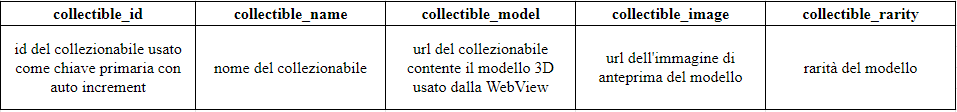
\includegraphics[width=\textwidth]{collectibles}   
    Figure 1: Tabella dei collezionabili
\end{center}

\medskip

\begin{center}
    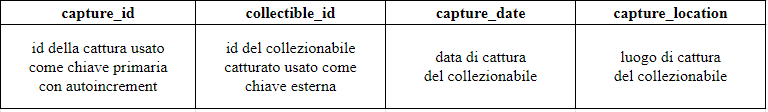
\includegraphics[width=\textwidth]{captures}   
    Figure 2: Tabella delle catture
\end{center}

\subsection{Inserimento dei collezionabili nel database}

Quando l'applicazione viene avviata, la classe MainActivity mette in esecuzione un Thread che implementa l'interfaccia \textbf{DownloadThread}.
Quest'ultimo si occupa di scaricare dalla rete la lista di collezionabili che l'utente può catturare e li inserisce all'interno del database.

La RestAPI fornisce due differenti endpoint:
\begin{itemize}
    \itemsep 0em 
    \item \href{https://backend.voxel.frangioniwebdev.com/api.php?endpoint=models/list}{endpoint=models/list}, contiene la lista di tutti i collezionabili
    da inserire all'interno del database. La lista è rappresentata in formato JSON.
    \item \href{https://backend.voxel.frangioniwebdev.com/db-version}{endpoint=db-version}, contiene la versione del database lato server. Questo endpoint
    viene contattato dal Thread per sapere se deve scaricare nuovi collezionabili o meno.
\end{itemize}

Se è la prima volta che l'utente avvia l'applicazione, quindi non ha mai scaricato un collezionabile fino ad ora, il Thread contatta l'endpoint
\href{https://backend.voxel.frangioniwebdev.com/api.php?endpoint=models/list}{endpoint=mo-dels/list}, deserializza la lista in formato JSON inviata dal server
ed inserisce i collezionabili all'interno del database. 

Successivamente il Thread contatta l'endpoint \href{https://backend.voxel.frangioniwebdev.com/db-version}{endpoint=db-version}
e salva la versione del database (rappresentata come intero) in un file situato nella memoria interna del telefono.

\medskip

Se l'utente ha già avviato l'applicazione in passato e ha quindi già scaricato dei collezionabili dal server, il Thread contatta prima l'endpoint 
\href{https://backend.voxel.frangioniwebdev.com/db-version}{endpoint=db-version} e verifica se la versione del database del server è la stessa di quella
che ha memorizzato all'interno del telefono. Se le due versioni coincidono, significa che il server non ha fatto modifiche al database e quindi non è
necessario scaricare la lista di collezionabili. 

Se le due versioni sono differenti, significa che ci sono dei nuovi collezionabili da inserire nel database. A questo punto il Thread contatta l'endpoint
\href{https://backend.voxel.frangioniwebdev.com/api.php?endpoint=models/list}{endpoint=mo-dels/list}, scarica i nuovi collezionabili e aggiorna 
il file contenente in memoria la versione del database.

\subsection{Funzionamento della WebView}

Come descritto precedentemente, la WebView viene utilizzata all'interno del FragmentCollectible per visualizzare il modello 3D del collezionabile.

Per risparmiare il consumo di risorse di rete, la WebView implementa al suo interno un meccanismo di caching. Quest'ultimo è fornito internamente da 
Android. Attraverso il metodo \textbf{webSettings.setCacheMode()}, infatti, è possibile stabilire quale tipo di cache voler utilizzare per lo scaricamento della 
pagina web. Poichè il modello 3D una volta scaricato non cambia, è stato scelto di implementare come politica di cache \textbf{WebSettings.LOAD\texttt{\_}CACHE\texttt{\_}
ELSE\texttt{\_}NETWORK}. In questo modo, se la pagina web è presente in cache, allora verrà visualizzata senza dover scaricare la pagina dalla rete.

\medskip

L'\href{https://voxel.frangioniwebdev.com/?model=adventure-time&mode=light}{url} che la pagina web contatta contiene due parametri di richiesta in GET:
\begin{itemize}
    \itemsep 0em 
    \item \textbf{model=[nome-modello]}, serve per decidere quale modello 3D renderizzare a schermo
    \item \textbf{mode=[light / dark]}, serve per cambiare il colore di sfondo della pagina web. Viene utilizzato per la modalità chiara o scura del telefono.
\end{itemize}

\subsection{Funzionamento della Mappa}

I collezionabili vengono generati in maniera randomica attorno all'utente e la loro posizione rimane in memoria finché
l'applicazione non viene chiusa. Quando l'utente si muove nella mappa, dopo una certa distanza, i collezionabili più lontani vengono
rimossi e vengono nuovamante generati attorno al giocatore. L'utente non ha la possibilità di muovere la telecamera, ma essa è bloccata sulla sua
posizione e segue tutti i suoi spostamenti. I collezionabili sono rappresentati sotto forma di Marker e vengono gestiti dalla classe \textbf{MarkerHandler}.

\medskip

La classe MarkerHandler si occupa di gestire la creazione, la generazione e la cattura dei collezionabili, rappresentati
all'interno della mappa come Marker.
Per tenere in memoria la posizione dei Marker sulla mappa anche quando l'utente cambia schermata, muovendosi per esempio fra
i vari Fragment dell'applicazione, è stato deciso di implementare una classe di tipo Singleton. In questo modo la classe MarkerHandler
rimane in memoria e non viene distrutta dal GarbageCollector, finché l'utente (o il sistema) non decide di terminare l'applicazione.

\medskip

Per catturare un collezionabile, è quindi sufficiente: cliccare su un Marker, premere sul menù a tendina che compare dopo aver cliccato e 
se l'utente è abbastanza vicino, il collezionabile viene catturato e il Marker rimosso dalla mappa.  

Come descritto nella documentazione, tutto il Funzionamento della mappa viene implementato all'interno del metodo \textbf{onMapReady()}, 
quest'ultimo invocato da una chiamata asincrona dal metodo \textbf{getMapAsync();}

il metodo onMapReady(), presente all'interno del FragmentMap, implementa 4 metodi:
\begin{itemize}
    \itemsep 0em 
    \item \textbf{updateLocationUI()}, modifica l'aspetto, le impostazioni e registra i listener della mappa
    \item \textbf{getLocationPermission()}, controllo i permessi di geolocalizzazione. Se non presenti, viene mostrata la richiesta di autorizzazione a schermo
    \item \textbf{getDeviceLocation()}, se l'utente ha conferito i permessi di geolocalizzazione, questo metodo tramite callback si occupa di
    prendere la posizione dell'utente
    \item \textbf{getMarkersLocation()}, se l'utente ha conferito i permessi di geolocalizzazione, quest metodo si occupa di generare i Marker attorno all'utente
\end{itemize}

\end{document}

